%!TeX jobName=challenges/stego/unified
%\nofiles
% Created by Bonita Graham
% Last update: February 2019 By Kestutis Bendinskas
%https://es.overleaf.com/gallery/tagged/academic-journal
% Authors:
% Please do not make changes to the preamble until after the solid line of %s.

\documentclass[letterpaper,10pt]{article}
\usepackage[utf8]{inputenc} % Codificación UTF-8
\usepackage[explicit]{titlesec}
\setlength{\parindent}{0pt}
\setlength{\parskip}{1em}
\usepackage{hyphenat}
\usepackage{ragged2e}
%Para colocar puntos en los itemes especiales
\usepackage{pifont}
\RaggedRight

% These commands change the font. If you do not have Garamond on your computer, you will need to install it.
%\usepackage{garamondx}
\usepackage[T1]{fontenc}
\usepackage{amsmath, amsthm}
\usepackage{graphicx}

% This adjusts the underline to be in keeping with word processors.
\usepackage{soul}
\setul{.6pt}{.4pt}


% The following sets margins to 1 in. on top and bottom and .75 in on left and right, and remove page numbers.
\usepackage{geometry}
\geometry{vmargin={1in,1in}, hmargin={.75in, .75in}}
\usepackage{fancyhdr}
\pagestyle{fancy}
\pagenumbering{gobble}
\renewcommand{\headrulewidth}{0.0pt}
\renewcommand{\footrulewidth}{0.0pt}

% These Commands create the label style for tables, figures and equations.
\usepackage[labelfont={footnotesize,bf} , textfont=footnotesize]{caption}
\captionsetup{labelformat=simple, labelsep=period}
\newcommand\num{\addtocounter{equation}{1}\tag{\theequation}}
\renewcommand{\theequation}{\arabic{equation}}
\makeatletter
\renewcommand\tagform@[1]{\maketag@@@ {\ignorespaces {\footnotesize{\textbf{Equation}}} #1.\unskip \@@italiccorr }}
\makeatother
\setlength{\intextsep}{10pt}
\setlength{\abovecaptionskip}{2pt}
\setlength{\belowcaptionskip}{-10pt}

\renewcommand{\textfraction}{0.10}
\renewcommand{\topfraction}{0.85}
\renewcommand{\bottomfraction}{0.85}
\renewcommand{\floatpagefraction}{0.90}

% These commands set the paragraph and line spacing
\titleformat{\section}
  {\normalfont}{\thesection}{1em}{\MakeUppercase{\textbf{#1}}}
\titlespacing\section{0pt}{0pt}{-10pt}
\titleformat{\subsection}
  {\normalfont}{\thesubsection}{1em}{\textit{#1}}
\titlespacing\subsection{0pt}{0pt}{-8pt}
\renewcommand{\baselinestretch}{1.15}

% This designs the title display style for the maketitle command
\makeatletter
\newcommand\sixteen{\@setfontsize\sixteen{16pt}{6}}
\renewcommand{\maketitle}{\bgroup\setlength{\parindent}{0pt}
\begin{flushleft}
\vspace{-.375in}
\sixteen\bfseries \@title
\medskip
\end{flushleft}
\textsc{\@author}\\
\textit{\today}
\egroup}
\makeatother

% This styles the bibliography and citations.
%\usepackage[biblabel]{cite}
\usepackage[sort&compress]{natbib}
\setlength\bibindent{2em}
\makeatletter
\renewcommand\@biblabel[1]{\textbf{#1.}\hfill}
\makeatother
\renewcommand{\citenumfont}[1]{\textbf{#1}}
\bibpunct{}{}{,~}{s}{,}{,}
\setlength{\bibsep}{0pt plus 0.3ex}




%%%%%%%%%%%%%%%%%%%%%%%%%%%%%%%%%%%%%%%%%%%%%%%%%

% Authors: Add additional packages and new commands here.
% Limit your use of new commands and special formatting.

% Place your title below. Use Title Capitalization.
\title{Write-up: HackTheBox - Stego - Unified}

% Add author information below. Communicating author is indicated by an asterisk, the affiliation is shown by superscripted lower case letter if several affiliations need to be noted.
\author{Sebastián Sepúlveda @piblack}


\pagestyle{empty}
\begin{document}

% Makes the title and author information appear.
\vspace*{.01 in}
\maketitle
\vspace{.12 in}

% Start the main part of the manuscript here.
% Comment out section headings if inappropriate to your discipline.
% If you add additional section or subsection headings, use an asterisk * to avoid numbering.

\textbf{Información:} Categoria Stego, 20 points.

\textbf{Descripción:} This file seems to contain innocuous information. What is the true message?

\section*{WriteUp}

Para comenzar descargamos el archivo de HackTheBox. Obtenemos el archivo \texttt{BOD\_30079.txt} que contiene lineas ilegibles.

\begin{figure}[h]
  \centering
  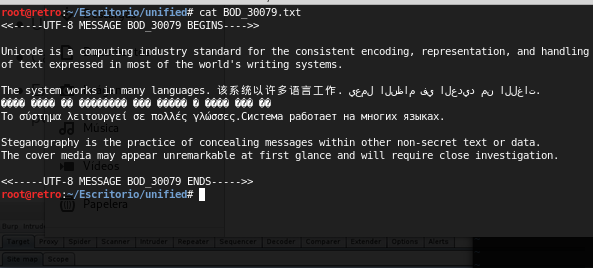
\includegraphics[scale=0.7]{images/unified/archivo_flag.png}
  \captionof{figure}{Copiando texto de Burpsuite}
  \label{fig:archivo}
\end{figure}

Para poder descifrarlas ocupamos \texttt{BurpSuite} que contiene una pestaña de decodificador de texto plano o hexadecimal.

\begin{figure}[h]
  \centering
  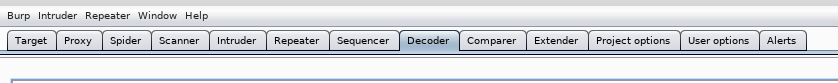
\includegraphics[scale=0.5]{images/unified/burpsuite.png}
  \captionof{figure}{Pestaña de Burpsuite}
  \label{fig:pestanha}
\end{figure}

Copiamos y pegamos el texto y encontramos el flag escondido. \textbf{Ver Figura \ref{fig:flag}}

\begin{figure}[h]
  \centering
  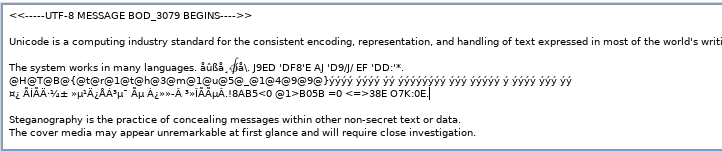
\includegraphics[scale=0.7]{images/unified/captura_flag.png}
  \captionof{figure}{Copiando texto de Burpsuite}
  \label{fig:flag}
\end{figure}

Con \texttt{$@H@T@B@{@t@r@1@t@h@3@m@1@u@5@_@1@4@9@9@}$} es cosa de quitar las $@$ y terminamos.

\textbf{Flag: }HTB{tr1th3m1u5\_1499}

\textbf{NOTA: }algo importante es copiar y pegar el texto desde el archivo de texto, pues copiandolo
desde la linea de comando el programa no va a poder leer el texto


\end{document}
